% !TeX root = ../master.tex

\lecture{4}{2026-09-15}{Conduction, Pt. III}

\subsection{Transient Heat Conduction}
In transient heat conduction, the temperature field changes with time,
\begin{equation*}
  T = T(x,y,z,t).
.\end{equation*}
The governing heat equation therefore retains the transient term
\begin{equation*}
  \rho c \frac{\partial T}{\partial t}.
.\end{equation*}

\subsubsection{Lumped System Analysis}
In heat transfer analysis, some bodies are observed to behave like a ``lump'', i.e. whose interior temperature remains uniform at any point during a heat transfer process.
The temperature of such bodies can be taken to be a function of time only, $T(t)$.
Analysis utilizing this idealization is known as \textit{lumped system analysis}.
This is often applicable for small bodies.

We consider a body of arbitrary shape of mass $m$, volume $\mathscr{V}$, surface area $A_s$, density $\rho$, and specific heat $c_p$ initially at uniform temperature $T_i$.
At time $t = 0$, the body is placed into a medium at temperature $T_{\infty}$, and heat transfer takes place between the body and the medium with heat transfer coefficient $h$.
We assume the system to be lumped, such that the temperature within the body remains uniform, $T = T(t)$.
During a differential time element $\mathrm{d}t$, the temperature of the body rises by a differential amount $\mathrm{d}T$.
An energy balance of the solid for the time interval $\mathrm{d}t$ can be expressed as
\begin{equation*}
  h A_s \left( T_{\infty}-T \right) \, \mathrm{d}t  = m c_p \, \mathrm{d}T
.\end{equation*}
Noting that $m = \rho \mathscr{V}$ and $\mathrm{d}T = \mathrm{d}(T-T_{\infty})$ since $T_{\infty} = \text{constant}$ the above can be rearranged as
\begin{equation*}
  \frac{\mathrm{d}(T-T_{\infty})}{T-T_{\infty}} = - \frac{h A_s}{\rho \mathscr{V} c_p} \, \mathrm{d}t
.\end{equation*}
integrating from $t = 0$, at which $T = T_i$ to a time $t$ at which $T = T(t)$ gives
\begin{equation*}
  \ln \frac{T(t) - T_{\infty}}{T_i - T_{\infty}} = - \frac{h A_s}{\rho \mathscr{V}c_p}t
.\end{equation*}
Rearranging we obtain
\begin{equation} \label{eq:lumpedtemp}
  T - T_{\infty} = (T_i - T_{\infty}) e^{-bt}
\end{equation}
where
\begin{equation*}
  b = \frac{h A_s}{\rho \mathscr{V} c_p} \quad \unit{\per\s}
\end{equation*}
is a positive quantity.
The reciprocal of $b$, is termed $\tau$ and is called the time constant defined as:
\begin{equation*}
  \tau = \frac{1}{b} = \frac{\rho c_p \mathscr{V}}{h A_s} \qquad \implies \qquad \theta = e^{- \frac{t}{\tau}}
.\end{equation*}


\paragraph{Heat Transfer Rate and Total Heat Transfer}
Once the temperature $T(t)$ at time $t$ is found from \Mref{eq:lumpedtemp}, the rate of convection heat transfer between the body and its environment at that time can be determined from Newton's law of cooling as
\begin{equation*}
  \dot{Q}(t) = h A_s \left( T(t) - T_{\infty} \right)
.\end{equation*}
The \textit{total amount} of heat transfer between the body and the surrounding medium over the time interval $t = 0$ to $t$ is simply the change in the energy content of the body:
\begin{equation*}
  Q = m c_p (T(t) - T_i)
.\end{equation*}
The amount of heat transfer reaches its upper limit when the body reaches the surrounding temperature, therefore the \textit{maximum} heat transfer between the body and its surroundings is
\begin{equation*}
  Q_{\text{max}} = m c_p (T_{\infty} - T_i)
.\end{equation*}


\subsubsection{Biot Number and Lumped-System Criterion}
Now, we must determine when lumped analysis is appropriate to use.
The first step in establishing such a criterion is to define a characteristic length as:
\begin{equation*}
  L_c = \frac{\mathscr{V}}{A_s}
\end{equation*}
and a dimensionless \textit{Biot number} $\mathrm{Bi}$ as
\begin{equation} \label{eq:biot}
  \mathrm{Bi} = \frac{h L_c}{k}
.\end{equation}
The characteristic length $L_c$ to be used in the Biot number for simple geometries in which heat transfer is one-dimensional, such as a large plane wall of thickness $2L$, a long cylinder of radius $r_o$, and a sphere of radius $r_o$ becomes $L$, $r_o / 2$, and $r_o / 3$, respectively.
The Biot number is the ratio of internal resistance of a body to heat conduction to its external resistance to heat convection. 
Therefore a small Biot number represents a small resistance to conduction and thus small temperature gradients within the body.

Lumped system analysis assumes a uniform temperature distribution throughout the body.
Thus lumped system analysis is exact when $\mathrm{Bi} = 0$ and approximate when $\mathrm{Bi} > 0$.
It is generally accepted that lumped system analysis is applicable if
\begin{equation*}
  \mathrm{Bi} \leq \num{0,1} 
.\end{equation*}


\subsubsection{One-Dimensional Transient Heat Conduction}
We now move on to transient heat conduction in non-lumped bodies one-dimensional bodies.
We now consider the variation of temperature with \textit{time} and \textit{position} in one-dimensional problems such as those associated with a large plane wall, a long cylinder, and a sphere.

\paragraph{Transient Conduction in a Plane Wall}
We consider a wall of total thickness $2L$.
The $x$-coordinate is measured from the centre plane, so $x = 0$ is the middle and $x = L$ is the exposed face.
The same fluid is on both sides.

\begin{figure} [ht]
  \centering
  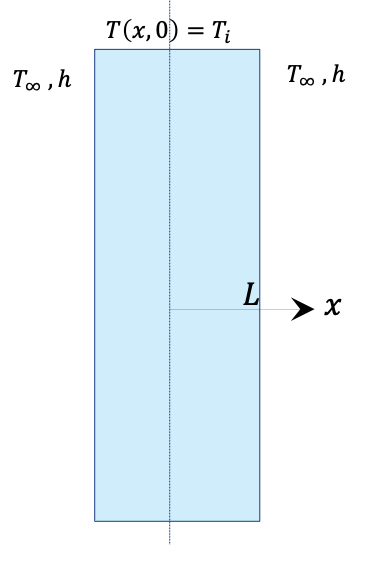
\includegraphics[width=0.7\linewidth]{./figures/transientwall.png}
  \caption{Transient Conduction in a Plane Wall.}
  \label{fig:transientwall}
\end{figure}

The left side at $x = 0$ is insulated (i.e. no heat leaves) and the right side $x = L$ loses heat to the environment through convection.
The initial state is everything starting at the same temperature.
Our governing differential equation is
\begin{equation*}
  \frac{\partial ^2 T}{\partial x^2}  = \frac{1}{\alpha} \frac{\partial T}{\partial t}, \qquad \alpha = \frac{k}{\rho c_p}
.\end{equation*}

\paragraph{Dimensionless Temperature, Biot Number and Fourier Number}
Solving the above equation with the given BC's and IC would give $T$ as a function of $x$, $t$, $T_i$, $T_{\text{inf}}$, $k$, $\alpha$, $h$ and $L$.
Instead, we can also opt to use dimensional analysis to make the problem dimension-less.
First, we define the dimensionless temperature:
\begin{equation*}
  \theta = \frac{T - T_{\infty}}{T_i - T_{\infty}}
\end{equation*}
this is the temperature excess.

We also define the Fourier number, $\mathrm{Fo}$:
\begin{equation*}
  \mathrm{Fo} = \frac{\alpha t}{L^2} = \frac{t}{L^2 / \alpha}
.\end{equation*}
The Fourier number can be seen as the ratio of elapsed time to the time required for heat to diffuse through the body.
So a small $\mathrm{Fo}$ means the process just started and a large $\mathrm{Fo}$ means diffusion has had a long time to act.

Using the Fourier and previously introduced Biot numbers the temperature excess of the wall can be written as:
\begin{equation*}
  \theta(x,t) = \frac{T - T_{\infty}}{T_i - T_{\infty}} = \underbracket{f_1 (\mathrm{Fo} \mathrm{Bi})}_{\text{Time part}} \cdot \underbracket{f_2 \left( \frac{x}{L}, \mathrm{Bi} \right)}_{\text{Position part}}
.\end{equation*}


\paragraph{One-Term Approximation}
The exact solution to the above is an infinite series.
For $\mathrm{Fo} > \num{0,2}$ is the first term of the series, however, normally enough.
Then:
\begin{align*}
  f_1(\mathrm{Fo}, \mathrm{Bi}) &\approx A_1 e^{-\lambda_1^2 \mathrm{Fo}} \\
  f_2 \left( \frac{x}{L}, \mathrm{Bi} \right) &\approx \cos \left( \lambda_1 \frac{x}{L} \right)
.\end{align*}
Meaning
\begin{equation*}
  \theta = \frac{T - T_{\infty}}{T_i - T_{\infty}} = A_1 e^{-\lambda_1^2 \cdot \mathrm{Fo}} \cdot \cos \left( \lambda_1 \frac{x}{L} \right)
\end{equation*}
where, $A_1$ and $\lambda_1$ are functions of $\mathrm{Bi}$ which are tabulated in \citepage{cengel2015heatmasstransfer}{Table 4--2}.

At the center of the wall, $x = 0$ the temperature $T_0$ is
\begin{equation*}
  \frac{T_0 - T_{\infty}}{T_i - T_{\infty}} = A_1 e^{-\lambda_1^2 \mathrm{Fo}}
.\end{equation*}
When the center temperature has been determined, the spatial part can be used:
\begin{equation*}
  T(x,t) - T_{\infty} = \left( T_0 (t) - T_{\infty} \right) \cos \left( \lambda_1 \frac{x}{L} \right)
.\end{equation*}
So first, one must use the initial temperature to determine how much the center has heated/cooled at time $t$ and then one uses the spatial profile to find the temperature near the surface or at any other point in the wall.

Instead of calculating the values of $A_1 e^{-\lambda_1^2 \mathrm{Fo}}$ and $\cos (\lambda_1 x / L)$ as shown above one can instead opt to read the values from so-called Heisler charts.
These are just lookup-plots for the above equations.

\paragraph{Total Heat Transfer}
In lumped systems the entire body has uniform temperature so the total heat transfer is easily found, however know the temperature varies with position $T = T(x,t)$.
In this case, the total energy change has to be integrated instead:
\begin{equation*}
  Q(t) = \int_{\mathscr{V}} \rho c \left( T(x,t) - T_i \right) \, \mathrm{d}\mathscr{V}
.\end{equation*}
After infinite time, the entire body reaches $T_{\infty}$ and therefore:
\begin{equation*}
  Q_{\mathrm{max}} = mc \left( T_{\infty} - T_i \right)
\end{equation*}
so $Q / Q_{\text{max}}$ tells the fraction of total energy transfer which has already happened.
For the plane wall one-term solution:
\begin{equation*}
  \frac{Q}{Q_{\text{max}}} = 1  - \theta_0 \frac{\sin \lambda_1}{\lambda_1}
.\end{equation*}
